\documentclass[final]{beamer}
\mode<presentation> {
    \usetheme{Berlin}
}

\usepackage[english]{babel}
\usepackage[utf8]{inputenc}

\usepackage{graphicx}
\usepackage{anyfontsize}
\usepackage{subcaption}
\usepackage{wrapfig}

\usepackage{color}
\definecolor{codegreen}{rgb}{0,0.6,0}
\definecolor{codegray}{rgb}{0.5,0.5,0.5}
\definecolor{codepurple}{rgb}{0.58,0,0.82}
\definecolor{backcolour}{rgb}{0.92, 0.92, 0.92}

\definecolor{titlecolor}{rgb}{0.2,0.2,0.2}
\definecolor{bodycolor}{rgb}{0.95,0.95,0.95}
\setbeamercolor*{block title}{fg=white, bg=titlecolor}
\setbeamercolor*{block body}{fg=black, bg=bodycolor}

\usepackage{listings}
\lstdefinestyle{python}{
    language = Python,
    commentstyle = \color{codegreen},
    basicstyle = \footnotesize,
    keywordstyle = \footnotesize,
    breakatwhitespace=false,
    breaklines = true,
    keepspaces = true,
    showspaces = false,
    showstringspaces = false,
    showtabs = false,
    tabsize = 2,
}

\usepackage[orientation=portrait,size=a0,scale=1.4,debug]{beamerposter}
\usepackage{tikz}

\setbeamertemplate{headline}{
    \begin{tikzpicture}[remember picture,overlay]
        \node[opacity=0.4] at (current page.north){
        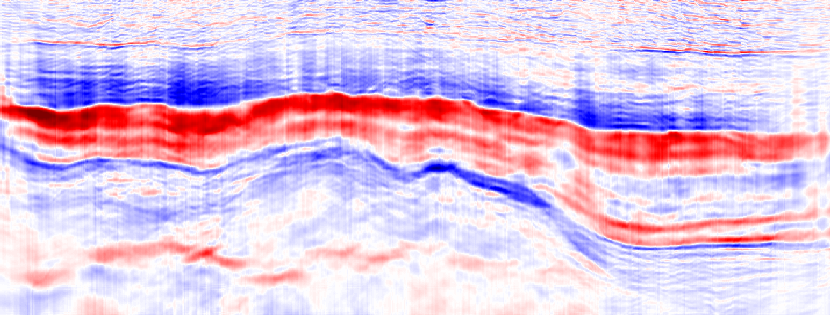
\includegraphics[width=\paperwidth]{volve.png}
    };
    \end{tikzpicture}
    \leavevmode

    \begin{beamercolorbox}[wd=\paperwidth]{headline}
        \vspace{4ex}\\
        \begin{columns}
            \begin{column}{.10\paperwidth}\end{column}
            \begin{column}{.60\paperwidth}
                \usebeamercolor{title in headline}{
                    \color{fg}\textbf{\fontsize{50mm}{50mm}\selectfont \inserttitle}\\[1ex]
                }
            \end{column}
            \begin{column}{.20\paperwidth}
                \hfill
                
\includegraphics[width=6cm]{py_logo.pdf}
                
\includegraphics[width=6cm]{c++.pdf}
            \end{column}
            \begin{column}{.10\paperwidth}
            \end{column}
        \end{columns}
        \vspace{16ex}\\
    \end{beamercolorbox}

    \begin{beamercolorbox}[wd=\paperwidth]{lower separation line head}
        \rule{0pt}{2pt}
    \end{beamercolorbox}
    \vskip-2cm
}


\setbeamertemplate{footline}{
    \begin{columns}%[t]
        \begin{column}{.40\paperwidth}
            \hspace{2cm}
            \color{fg}{\fontsize{20mm}{20mm}\selectfont {github.com/equinor/segyio}}\\[1ex]
            \hspace{2cm}
            \color{fg}{\fontsize{20mm}{20mm}\selectfont {Jørgen Kvalsvik jokva@equinor.com}}\\[1ex]
        \end{column}

        \begin{column}{.20\paperwidth}
        \end{column}

        \begin{column}{.20\paperwidth}
            
\includegraphics{equinor-red.eps}
            \hspace{.1\paperwidth}
        \end{column}
    \end{columns}

    \vspace{2cm}
}

%gets rid of bottom navigation bars
\setbeamertemplate{navigation symbols}{}

\title[segyio] {segyio}
\author[Kvalsvik]{Jørgen Kvalsvik}
\institute[Equinor]{Equinor}
\date{\today}

\newcommand{\horizontalpad}{2cm}
\newcommand{\verticalpad}{1.7cm}

\addtobeamertemplate{block begin} {}
    {\leftskip=\horizontalpad\rightskip=\horizontalpad\vspace{\verticalpad}}

\addtobeamertemplate{block end}
    {\vspace{\verticalpad}}
    {\vspace{2ex}}

\begin{document}

\begin{frame}{}
\begin{columns}[t]
\newcommand{\columnmargin}{0.45\textwidth}

\begin{column}{\columnmargin}
    \begin{block}{\large Introduction}
        Segyio is a fast library with a powerful Python interface for reading
        and writing data in SEG-Y and seismic-unix format. It supports many
        numerical formats, including IBM float, 4- and 8-byte IEEE float, and
        several integer sizes. All interfaces are designed to mirror common
        python data types (list, dict), which can be sliced and iterated over.
    \end{block}

    \begin{block}{\large Simple and free}
        Installing segyio is simple - Python packages are available for Linux,
        Windows and MacOS, and it is available in Debian and Ubuntu, in
        addition to distributions in source code form. It is licensed under the
        LGPL v3, and free to use for any purpose. To get segyio:

        \begin{description}[align=right,labelwidth=1cm]
            \item [\emph{pip}] pip install segyio
            \item [\emph{debian/ubuntu}] apt install python3-segyio
        \end{description}
    \end{block}

    \begin{block}{\large Geometry aware}
        It is quite common that SEG-Y files contain a single, post-stack survey
        with the traces sorted. Segyio can figure this out, and offers a
        convenient interface to read 2D lines (or ranges of lines) with just
        the line number.
        \begin{minipage}{0.9\textwidth}
            \vspace{1em}
            \lstinputlisting[style = python]{f3.py}
        \end{minipage}
    \end{block}
\end{column}

\begin{column}{\columnmargin}

    \begin{block}{\large Pure data, readily available}
        Numpy arrays is the primary data type in segyio, to give users the
        power and flexibility to solve problems in any domain. Segyio is not
        biased towards any particular domain, and is just as well suited for
        seismic processing, seismic interpretation, and even machine learning.
        Large files are supported - segyio has been used to write single files
        of 11TB of synthetic seismic.
    \end{block}

    \begin{block}{\large In action}
        Segyio alone only reads and writes SEG-Y and SU. However, because of
        its powerful Python interface, complex tasks can be solved with
        straight-forward code. For example, consider the use case of shrinking
        a file by removing all samples beyond a certain depth:

        \begin{minipage}{0.90\textwidth}
        \lstinputlisting[style = python, title = cut.py]{cut.py}

        \begin{figure}[c]
            \begin{subfigure}{0.40\textwidth}
                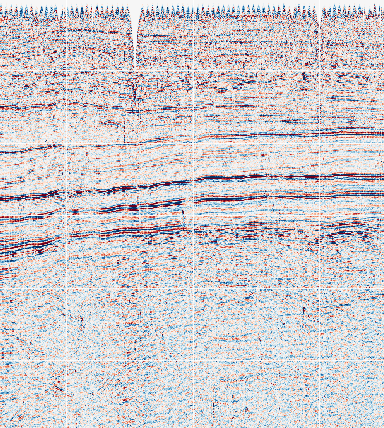
\includegraphics{pre-cut.png}
                \caption{src - before cut.py}
            \end{subfigure}
            ~
            \begin{subfigure}{0.40\textwidth}
                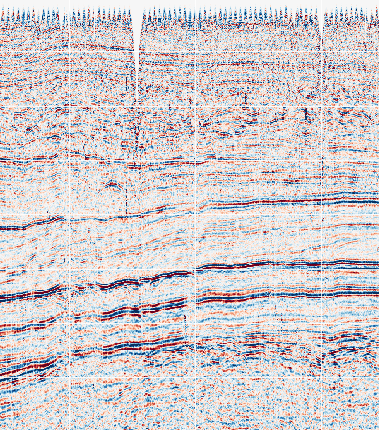
\includegraphics{post-cut.png}
                \caption{dst - after cut.py}
            \end{subfigure}
        \end{figure}
        \vspace{2ex}
        \end{minipage}

        Curated, in-depth, and interactive examples can be found at
        github.com/equinor/segyio-notebooks
    \end{block}
\end{column}

\end{columns}

\begin{center}
\begin{minipage}{0.9\paperwidth}

\begin{block}{\large Speed}
    \begin{columns}[t]
    \begin{column}{.6\textwidth}
        The core library is written in C and C++ for both portability and
        performance. This makes segyio very fast, even for large files.  The
        Python code only allocate memory and handle user input, such as
        translating slices into indices, and delegate the actual work to C and
        C++.

        When reading a trace in Python with \textbf{f.trace[traceno]}, C is
        used to compute the on-disk offset of the trace:

        \begin{equation*}
            \text{disk-offset}
                = 3600 \cdot (1 + n_\text{ext})
                + 400
                + (n_\text{samples} + 240) \cdot t_\text{traceno}
        \end{equation*}

        \begin{description}[align = right]
            \item [3600] size of textual headers
            \item [400] size of global binary header
            \item [240] size of trace headers
            \item [$n_\text{ext}$] number of extended textual headers
            \item [$n_\text{samples}$] samples-per-trace
        \end{description}

        Then, data is read from disk, and converted into native numericals if
        needed. This process is outlined in the figure on the right.
    \end{column}

    \begin{column}{.25\textwidth}
        \begin{figure}
            \includegraphics[width=\textwidth]{read-trace.eps}
            \label{fig:read-trace-graph}
        \end{figure}
    \end{column}
    \end{columns}
\end{block}

\end{minipage}
\end{center}

\end{frame}

\end{document}
